
\thispagestyle{empty}
\newpage
%%%%%%%%%%%%%%%%%%%%%%%%%%%%%%%%%%%%%%%%%%%%%%%%%%%%%%%%%%%%%%%%%%%%%%%%%%%%%%%%%%%%%%%%%%%%%%
%Fourth page - Start of the thesis
\setcounter{page}{3} 
\section{Introduzione}
In questa relazione si andrà ad esporre la procedura di dimensionamento di una briglia filtrante, da realizzare nel fiume Boite, quest'ultimo passante per Cortina d’Ampezzo.
Tale operazione di dimensionamento è costituita da tre parti: nella prima verrà calcolata la linea segnalatrice di possibilità pluviometrica (LSPP); successivamente, calcolato il tempo
di corrivazione, si andrà a ricavare il valore di portata di picco Q; infine, avverrà il calcolo di progetto della briglia.\\


 
\section{Descrizione del bacino e nozioni teoriche}

\subsection{Il fiume Boite ed il suo bacino}
Il fiume Boite è un corso idrico a carattere torrentizio delle Dolomiti. Le sue caratteristiche principali sono le seguenti:
\begin{itemize}
    \item lunghezza: 45.07 km;
    \item portata media: 12.71 $\frac{m^3}{s}$;
    \item area del bacino idrografico: 395.9 km$^2$;
    \item altitudine della sorgente: 1800 m s.l.m.;
\end{itemize}
Tale corso idrico è alimentato da diversi affluenti, e sfocia nel fiume Piave.
\cite{fiume_boite}
\subsection{La briglia filtrante}
Una briglia filtrante è una struttura antropica che viene posta lungo i corsi d'acqua montani.\\
L'obiettivo di tali opere è quello di consentire il passaggio dell'acqua del corso idrico, e di selezionare la quantità di sedimenti in movimento.\\
Per fare ciò, tali briglie possiedono:
\begin{itemize}
    \item una o più aperture nel corpo centrale;
    \item una "piazza di deposito" a monte, dove avviene il deposito dei detriti.
\end{itemize} 
Il ridotto passaggio di acqua attraverso le aperture (durante un evento di piena) riduce la velocità di flusso; ne deriva una minore capacità di trasporto di detriti, i quali vengono depositati.
\cite{prov_bolz}\\
Successivamente al picco di piena, la velocità di passaggio dell'acqua aumenta nuovamente, permettendo lo svuotamento dai detriti della "piazza di deposito".

\subsection{Linea segnalatrice di probabilità pluviometrica}
La linea segnalatrice di probabilità pluviometrica è un parametro matematico che riguarda gli eventi di precipitazione.\\
Tale funzione mette in relazione la quantità massima di evento pluviometrico, la sua durata ed il suo tempo di ritorno. \\
La LSPP si ricava andando ad elaborare i dati storici di precipitazione accaduti in un particolare territorio: la curva risultante sarà caratteristica di quel dato luogo.\\
La procedura di calcolo della LSPP si articola in diversi passaggi. \\
Come primo passaggio occorre andare ad ordinare i valori storici di precipitazione, in ordine crescente. Dopo aver fatto ciò, si assegna ad ogni valore la propria plotting position, attraverso la formula di Weibull:
\begin{equation}
\label{P_em}
    P_{em}=\frac{i}{N+1}
\end{equation}
Tale formula permette di valutare la probabilità di non superamento di un fenomeno, solamente valutando la sua disposizione in una serie di dati.\\
Successivamente, dai dati storici di precipitazione si ricavano i parametri statistici di media e deviazione standard, rispettivamente secondo le successive formule:
\begin{equation}
\label{media_aritmetica}
    m = \frac{x_1+x_2+...+x_N}{N}
\end{equation}
\begin{equation}
\label{dev.st}
    \sigma = \sqrt{\frac{\Sigma(X_1 - \mu)^2}{N+1}}
\end{equation}
Da questi due valori statistici si calcolano i parametri della distribuzione F(y), ovvero $\alpha$ e $u$, mediante il metodo dei momenti:
\begin{equation}
\label{alpha}
\alpha = \frac{\sqrt{6} \cdot \sigma}{\pi}    
\end{equation}
\begin{equation}
\label{u}
    u = \bar{h} - 0.5772 \cdot \alpha
\end{equation}
Conoscendo questi parametri è possibile ricavare la variabile ridotta $y = \frac{\bar{h}-u}{\alpha}$, che permette finalmente di trarre la funzione della distribuzione di Gumbel:
\begin{equation}
  F(y) = e^{e^{-y}}
\end{equation}
E' possibile creare un grafico che metta in relazione l'altezza di precipitazione h (in ordinata) e la relativa variabile ridotta ricavata dai calcoli (in ascissa): facendo ciò si adatta la distribuzione di probabilità di Gumbel.
\begin{figure}[H]
    \centering
    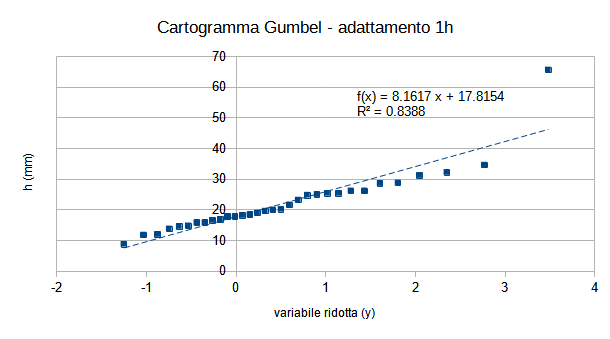
\includegraphics[width=0.7 \textwidth]{immagini/cartogramma_gumbel_1h.png}
    \caption{Cartogramma di Gumbel, con adattamento di precipitazioni di 1 ora di durata.}
    \label{fig:cartogramma_gumbel_1h}
\end{figure}
Il programma con cui è stato ricavato questo grafico (Excel) permette di conoscere la funzione della linea di tendenza, e del relativo valore di $R^2$. \\
Il valore $R^2$, anche detto "Coefficiente di determinazione" è un parametro statistico che permette di misurare il legame tra la variabilità dei dati e la correttezza del modello statistico utilizzato. \cite{r_quadro} \\
Successivamente, è possibile procedere al confronto grafico tra la probabilità empirica P di Weibull e la F(h):
\begin{figure}[H]
    \centering
    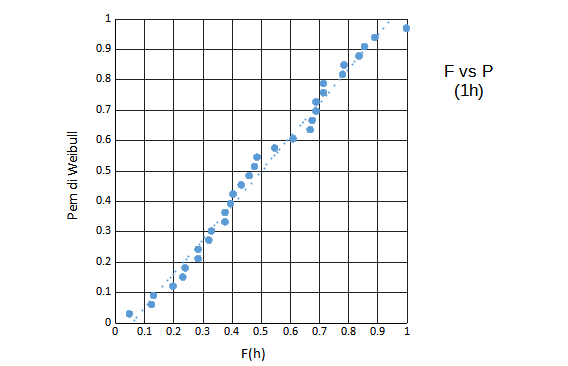
\includegraphics[width=0.7 \textwidth]{immagini/f_vs_p_1h.png}
    \caption{Confronto grafico tra la probabilità empirica di Weibull e la probabilità F(h).}
    \label{fig:f_vs_p_1h}
\end{figure}
La disposizione dei punti attorno la bisettrice permette di intuire come i valori di probabilità siano congruenti reciprocamente.\\
Un altro indicatore con cui è possibile valutare la concordanza di probabilità è il $\chi ^2$. Infatti, tale parametro statistico permette di verificare se le frequenze dei valori osservati si adattano a quelle teoriche, di una distribuzione di probabilità prefissata.\\
Al fine di confermare la coerenza tra le probabilità, il valore del $\chi ^2$ calcolato dev'essere inferiore a quello teorico.\\
Per esempio, nel caso di adattabilità di 1h: 
\begin{itemize}
    \item $\chi ^2$ calcolato: 3.9375
    \item $\chi ^2$ teorico: 5.9915
\end{itemize}
Al fine di conoscere la precipitazione prevista ($h_t$) per un certo tempo di ritorno, occorre valutare la relativa linea segnalatrice di possibilità pluviometrica.\\
Per fare ciò, si utilizzerà la formula 
\begin{equation}
    y_{t}= -\ln \left[ \ln \left(\frac{1}{F(h)} \right) \right] \rightarrow y_{t}= -\ln \left[ \ln \left(\frac{T}{T-1} \right) \right]
    \label{variabile_ridotta}
\end{equation}
Dopo aver trovato il parametro $y_t$, si andrà a ricavare $h_t$ mediante la successiva formula:
\begin{equation}
h_t = u + \alpha \cdot y_t    
\label{h_t}
\end{equation}
Questi calcoli potranno essere ripetuti per ogni fascia oraria disponibile e per qualsiasi tempo di ritorno.\\
Per esempio, la linea segnalatrice di possibilità pluviometrica del nostro bacino, per un tempo di ritorno di 10 anni, è la seguente.
\begin{figure}[H]
    \centering
    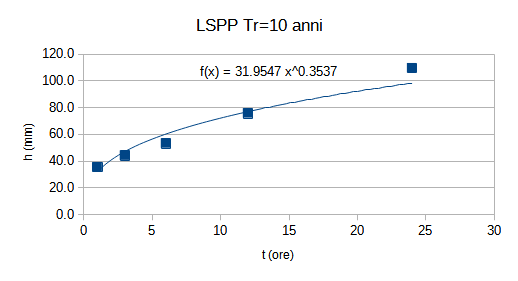
\includegraphics[width=0.7 \textwidth]{immagini/lspp_10anni.png}
    \caption{Linea segnalatrice di probabilità pluviometrica del bacino del fiume Boite, per tempo di ritorno di 10 anni.}
    \label{fig:lspp_10anni}
\end{figure}
Anche per questo caso, il programma che ha permesso il calcolo permette di inserire la funzione matematica della linea di tendenza, che in questo caso è $h_{10}= 31.9547 \cdot x^{0.3537}$. \\
Da tale espressione è possibile conoscere l'altezza di precipitazione di qualsiasi durata (possibilmente inferiore alle 24 ore), per tempo di ritorno di 10 anni. Infatti, nella formula l'incognita è rappresentata dal tempo di durata dell'evento di pioggia.

\subsection{Calcolo della portata di picco}
Lo studio della portata di picco è essenziale per conoscere la massima quantità d'acqua in movimento nel bacino, soprattutto nel caso in cui la durata di un evento pluviometrico eguagli il tempo di corrivazione del bacino.\\
Infatti, è proprio questa la peggiore condizione idraulica, poichè:
\begin{itemize}
    \item all'aumentare della durata di precipitazione l'intensità non aumenta in modo direttamente proporzionale;
    \item al diminuire della durata di precipitazione l'altezza di pioggia è direttamente proporzionale.
\end{itemize}
La funzione che permette di conoscere la portata di picco ($Q_p$) è la seguente:
\begin{equation}
    Q_p = C_d \cdot \frac{h_r \cdot A}{t_c}
    \label{Qp}
\end{equation}
dove: 
\begin{itemize}
    \item $C_d$ è il coefficiente di deflusso;
    \item $h_r(t_c, T_r)$ è l'altezza di pioggia corrispondente al tempo di corrivazione $t_c$ ed al tempo di ritorno $T_r \rightarrow h_r = a \cdot t_c ^n$;
    \item $A$ è l'area del bacino.
\end{itemize}
\subsubsection*{Il tempo di corrivazione}
Il tempo di corrivazione di un bacino ($t_c$) è il tempo massimo che impiega una goccia per attraversare completamente il bacino, fino ad arrivare alla sezione di chiusura.\\
Tale tempo di passaggio può essere calcolato in diversi modo, per questa relazione è stata utilizzata la formula di Giandotti:
\begin{equation}
    t_c = \frac{4 \sqrt{A} + 1.5 \cdot L}{0.8 \cdot \sqrt{z}}
    \label{giandotti}
\end{equation}
dove: 
\begin{itemize}
    \item $A$ è l'area del bacino, in $km^2$;
    \item $L$ è la lunghezza dell'asta principale, in $km$;
    \item $z$ è l'altezza media del bacino rispetto alla sezione di chiusura, espressa in $m$.
\end{itemize}
\subsubsection*{Il coefficiente di deflusso}
Il coefficiente di deflusso è il rapporto tra la precipitazione efficace del bacino e la precipitazione totale. Offre in maniera generale una rappresentazione del deflusso superficiale e dell'infiltrazione del bacino.\\
La formula è quindi:
\begin{equation}
    C_d = \frac{P_e}{h_r}
    \label{Cd}
\end{equation}
\subsubsection*{La precipitazione efficace}
La precipitazione efficace equivale alla quantità d'acqua dell'evento meteorico, al netto delle perdite iniziali e dell'imbibimento del terreno. In pratica è la frazione di precipitazione che si trasforma in deflusso superficiale.\\
Tale valore varia in base alle condizioni del terreno ed in funzione delle caratteristiche del territorio.\\
La formula per calcolare la precipitazione efficace è la seguente: 
\begin{equation}
    P_e = \frac{(h_r - I_a)^2}{h_r - I_a + S}
    \label{Pe}
\end{equation}
dove la lettera $S$ indica lo storage idrico del terreno, che può essere calcolato mediante: 
\begin{equation}
    S = S_0 \cdot \left ( \frac{100}{CN} -1 \right )
    \label{storage}
\end{equation}
Nella precedente funzione, la costante $S_0$ equivale a 254 mm ed il valore CN quantifica la permeabilizzazione del suolo.

\subsection{Progetto della sezione di un canale}
Generalmente, in assenza di vincoli esterni e tecnici, durante il dimensionamento di un canale si adotta la sezione di minima resistenza, ovvero quella sezione che a parità di area permette la velocità media massima, e quindi la portata massima.\\
A parità di altre condizioni, la velocità media dipende dal valore di raggio idraulico (e quindi dalla forma e dimensione della sezione).
\subsubsection*{Calcolo della profondità di moto uniforme $y_1$}
Il parametro $y_1$ indica la profondità del canale con cui la portata $Q$ viene convogliata con la sezione di minor perimetro bagnato.\\
Il calcolo della profondità critica è un metodo iterativo, ovvero il risultato finale si ottiene dalla ripetizione di una serie di calcoli.
Il procedimento inizia con il calcolo di una profondità di primo tentativo $y_0$, mediante la seguente equazione:
\begin{equation}
    y_0 = \left ( \frac{Q}{B \cdot K_S \cdot \sqrt{i_F}} \right) ^ {\frac{3}{5}}
    \label{prof_critica_tentativo}
\end{equation} 
Successivamente si calcola il relativo raggio idraulico, mediante la formula:
\begin{equation}
    Rh_0 = \frac{B \cdot y_0}{B + 2\cdot y_0}
    \label{raggio_idraulico}
\end{equation} 
E da questo raggio idraulico si calcola nuovamente l'altezza $y$:
\begin{equation}
    y_1 = \frac{Q}{B \cdot K_S \cdot R_h ^\frac{2}{3} \cdot \sqrt{i_F}}
    \label{prof_critica}
\end{equation} 
Nel caso che la differenza percentuale tra le due profondità è inferiore al 2\%, il processo può terminare; in caso contrario, occorre ripetere i procedimenti, calcolando il raggio idraulico mediante l'ultima profondità critica ottenuta.
\begin{equation}
    \frac{|y_1 - y_0|}{y_0} \le 2\%
    \label{scostamento_prof_critica}
\end{equation} 
\subsubsection*{Calcolo della $H$ del canale}
Avendo i valori di $y_c$ (calcolata) e di $B$ (di progetto), è possibile calcolare il valore $H$, ovvero l'energia specifica del canale.
La formula per calcolare $H$ è la seguente: 
\begin{equation}
    H = y + \frac{q^2}{2 \cdot g \cdot y^2}
    \label{energia_specifica_canale}
\end{equation} 
Il parametro $q$ indica la portata del canale per unità di larghezza, e si calcola con $q = \frac{Q}{B}$.
\subsubsection*{Calcolo della larghezza limite $B_L$, per il passaggio in condizioni critiche}
Il valore $B_L$, ovvero la larghezza della sezione rettangolare della briglia, in condizioni critiche, si calcola con la seguente formula:
\begin{equation}
    B_L = \frac{Q}{0.414 \cdot \sqrt{g} \cdot H_1 ^{1.5}}
    \label{larghezza_specifica}
\end{equation}
\section{Elaborazione dati}
I seguenti procedimenti di calcolo interessano valori valutati per un tempo di ritorno di 50 anni.\\
In questo capitolo verranno effettuati i calcoli di progetto, in concordanza con le nozioni teoriche esposte nella sezione precedente.\\
Per semplificare l'esposizione, verranno mostrati solamente i calcoli per eventi pluviometrici di 1 ora di durata. Ovviamente i calcoli sono stati ripetuti per ogni durata di evento pluviometrico (1, 3, 6, 12 e 24 ore), per il tempo di ritorno di 50 anni.
\subsection{Dati storici di precipitazione}
% Please add the following required packages to your document preamble:
% \usepackage{multirow}
\begin{table}[H] \centering \footnotesize
\begin{tabular}{cccccc}
\multirow{3}{*}{\textbf{Anno}} & \multicolumn{5}{l}{\textbf{Pioggia in mm}}                                           \\
\toprule
                               & \textbf{1 ora} & \textbf{3 ore} & \textbf{6 ore} & \textbf{12 ore} & \textbf{24 ore} \\
                               & \textbf{mm}    & \textbf{mm}    & \textbf{mm}    & \textbf{mm}     & \textbf{mm}     \\
\midrule
1992                           & 14.6           & 21             & 33.2           & 60.8            & 78              \\
1993                           & 18.4           & 23.4           & 41.8           & 65.4            & 76.6            \\
1994                           & 19.6           & 34.4           & 47.2           & 64.8            & 83.2            \\
1995                           & 15.8           & 19.6           & 32             & 41.6            & 51              \\
1996                           & 24.8           & 31             & 40             & 64.8            & 100             \\
1997                           & 28.6           & 36             & 36             & 55.6            & 69              \\
1998                           & 17.8           & 28.2           & 39             & 55.2            & 78              \\
1999                           & 11.8           & 30.2           & 48.4           & 81.4            & 96.4            \\
2000                           & 15.8           & 25.4           & 46.4           & 67.8            & 73.4            \\
2001                           & 25.4           & 46.2           & 50.6           & 61.8            & 72              \\
2002                           & 17.8           & 31.6           & 40             & 63.6            & 98.8            \\
2003                           & 21.6           & 25.4           & 41.6           & 71.6            & 91.2            \\
2004                           & 13.8           & 21             & 33.4           & 36.6            & 48.2            \\
2005                           & 26.2           & 31.4           & 37.2           & 50.4            & 69.8            \\
2006                           & 14.8           & 27.2           & 48.4           & 63.8            & 69.6            \\
2007                           & 32.2           & 43.4           & 44.8           & 50.8            & 78.2            \\
2008                           & 19             & 23.8           & 38.6           & 58.4            & 72              \\
2009                           & 20             & 25.8           & 34             & 53.6            & 95.4            \\
2010                           & 8.8            & 18.2           & 30.2           & 47              & 78.4            \\
2011                           & 25             & 27.2           & 31.4           & 49.6            & 81.8            \\
2012                           & 18.2           & 28.2           & 49.8           & 83              & 104             \\
2013                           & 16.8           & 22             & 39             & 61.8            & 69.2            \\
2014                           & 31.2           & 32.4           & 44             & 73.4            & 114.8           \\
2015                           & 20.2           & 25.4           & 36.8           & 42.8            & 50.2            \\
2016                           & 12             & 28.8           & 46.2           & 63              & 67.8            \\
2017                           & 25.4           & 29.2           & 36             & 62.6            & 72.4            \\
2018                           & 65.6           & 73             & 73.4           & 87              & 146.4           \\
2019                           & 16.6           & 24.2           & 42             & 60.4            & 85.6            \\
2020                           & 28.8           & 37.4           & 47.8           & 65.8            & 120.6           \\
2021                           & 26.2           & 37.4           & 45.6           & 51.6            & 54.6            \\
2022                           & 23.2           & 38             & 44             & 44.6            & 46.6            \\
2023                           & 34.6           & 35.4           & 52.2           & 67.4            & 96.2       \\
\bottomrule
\end{tabular}
\end{table}
\subsection{Calcolo della LSPP}
Successivamente ad aver ordinato in ordine crescente le altezze di precipitazione, si è assegnato ad ogni evento pluviometrico un indice di Weibull, mediante la formula \ref{P_em}.
Dopo aver fatto ciò, si calcolano i parametri statistici di media e deviazione standard, rispettivamente mediante le formule \ref{media_aritmetica} e \ref{dev.st}. \\

\begin{equation}
      m = \frac{x_1+x_2+...+x_N}{N} = \frac{8.8+...+65.6}{32} = 22.21 mm
\end{equation}
\begin{equation}
      \sigma = \sqrt{\frac{\Sigma(X_1 - \mu)^2}{N+1}}= \sqrt{\frac{(8.8 - 22.21)^2+...(65.6-22.21)^2}{32+1}} = 10.13 mm
\end{equation}
E da questi valori appena calcolati, ci si calcola i parametri della distribuzione F(y), utilizzando le formule \ref{alpha} e \ref{u}:
\begin{equation}
    \alpha = \frac{\sqrt{6} \cdot \sigma}{\pi} = \frac{\sqrt{6} \cdot 22.21}{\pi} = 7.90
\end{equation}
\begin{equation}
    u = \bar{h} - 0.5772 \cdot \alpha = 10.13- 0.5772 \cdot 7.90 = 17.65
\end{equation}
Successivamente, si effettua il calcolo della variabile ridotta, rispetto al tempo di ritorno, come secondo la formula \ref{variabile_ridotta}:
\begin{equation}
y_{t}= -\ln \left[ \ln \left(\frac{T}{T-1} \right) \right] = -\ln \left[\ln \left( \frac{50}{50-1} \right) \right ] = 3.902
\end{equation}
Ed infine si calcola l'altezza di precipitazione per il dato tempo di ritorno, utilizzando la formula \ref{h_t}:
\begin{equation}
h_t = u + \alpha \cdot y_t  = 17.65 + 7.90 \cdot 3.902= 48.5mm
\end{equation}
Infine, si effettua il test del $\chi^2$, che per semplicità verrà svolto dall'apposita funzione di Excel. I risultati sono i seguenti: 
\begin{itemize}
    \item $\chi ^2$ calcolato: 3.9375
    \item $\chi ^2$ teorico: 5.9915
\end{itemize}
\subsection{Calcolo della portata di picco} \label{portatadipicco}
Le caratteristiche del bacino sono le seguenti:
\begin{itemize}
    \item differenza totale di quota: 1000 m;
    \item CN: 85;
    \item area del bacino: 4 km$^2$;
    \item lunghezza dell'asta principale: 4 km;
    \item pendenza del reticolo idraulico (i$_f$): 0.025.
\end{itemize}
Utilizzando la formula di Giandotti \ref{giandotti} calcolo il tempo di corrivazione del reticolo (t$_c$):
\begin{equation}
    t_c = \frac{4 \sqrt{A} + 1.5 \cdot L}{0.8 \cdot \sqrt{z}} = \frac{4 \sqrt{4} + 1.5 \cdot 4}{0.8 \cdot \sqrt{1000}} = 0.48 h
\end{equation}
Al fine di conoscere la quantità di precipitazione efficace, per conoscere il coefficiente di deflusso, occorre quantificare lo storage idrico del suolo. Per fare ciò utilizzo la formula \ref{storage}
\begin{equation}
    S = S_0 \cdot \left ( \frac{100}{CN} -1 \right ) = 254 \cdot \left ( \frac{100}{85} - 1 \right) = 44.82mm
\end{equation}
Da questo parametro è possibile calcolare la precipitazione efficace, mediante la formula \ref{Pe}:
\begin{equation}
    P_e = \frac{(h_r - I_a)^2}{h_r - I_a + S} = \frac{(33.87 - 0.1 \cdot44.82)^2}{33.87 - 0.1\cdot48.82 + 48.82}= 11.64 mm
\end{equation}
Da questi valori è possibile calcolare il coefficiente di deflusso del bacino, mediante la formula \ref{Cd}:
\begin{equation}
    C_d = \frac{P_e}{h_r} = \frac{11.64}{33.87}= 0.36
\end{equation}
Infine, si calcola la portata di picco del reticolo idrografico del bacino, utilizzando la formula \ref{Qp}:
\begin{equation}
    Q_p = C_d \cdot \frac{h_r \cdot A}{t_c} = 0.36 \cdot \frac{33.87 \cdot 4 \cdot 1000}{0.48 \cdot 3600} = 26.82 \frac{m^3}{s}
\end{equation}

\subsection{Dimensionamento della sezione del canale} 
\subsubsection*{Profondità di moto uniforme}
Mediante la formula \ref{prof_critica_tentativo} si calcola la profondità critica di primo tentativo:
\begin{equation}
    y_0 = \left ( \frac{Q}{B \cdot K_S \cdot \sqrt{i_F}} \right) ^ {\frac{3}{5}} = \left ( \frac{26.82}{3 \cdot 10 \cdot \sqrt{0.025}} \right) ^ {\frac{3}{5}} = 2.83m
\end{equation} 
Successivamente si calcola il raggio idraulico equivalente, mediante la formula \ref{raggio_idraulico}:
\begin{equation}
    Rh_0 = \frac{B \cdot y_0}{B + 2\cdot y_0} = \frac{3 \cdot 2.83}{3 + 2\cdot 2.83} = 0.98 m
\end{equation} 
Da questo raggio idraulico si ricalcola la profondità critica, mediante la formula \ref{prof_critica}:
\begin{equation}
    y_1 = \frac{Q}{B \cdot K_S \cdot R_h ^\frac{2}{3} \cdot \sqrt{i_F}} = \frac{26.82}{3 \cdot 10 \cdot 0.98 ^\frac{2}{3} \cdot \sqrt{0.025}} = 5.73m
\end{equation} 
Infine, si calcola lo scostamento tra le profondità critiche ricavate, mediante la formula \ref{scostamento_prof_critica}:
\begin{equation}
    \frac{|y_1 - y_0|}{y_0} = \frac{|5.13 - 2.83|}{2.83} = 1.02  
\end{equation} 
Il risultato ottenuto è superiore al limite del 2\%; occorrà ripetere i calcoli, valutando nuovamente il raggio idraulico di un canale con altezza critica di 5.73 m.

\subsubsection*{Energia specifica}
Mediante la formula \ref{energia_specifica_canale} si calcola l'energia specifica del canale:
\begin{equation}
    H = y + \frac{q^2}{2 \cdot g \cdot y^2} = 5.13 + \frac{8.939^2}{2 \cdot 9.81 \cdot 5.13^2} = 5.285m
\end{equation} 

\subsubsection*{Larghezza limite}
Mediante la formula \ref{larghezza_specifica} si calcola la larghezza limite del canale, per il passaggio dell'acqua in condizione critica:
\begin{equation}
    B_L = \frac{Q}{0.414 \cdot \sqrt{g} \cdot H_1 ^{1.5}} = \frac{26.82}{0.414 \cdot \sqrt{9.81} \cdot 5.285 ^{1.5}} = 1.702m
\end{equation}
\section{Risultati}
In questo capitolo verranno esposti i risultati dei calcoli, relativi all'altezza di precipitazione per un assegnato tempo di ritorno, per la portata di picco e per il dimensionamento del canale.
\subsection{Altezza di precipitazione}
\begin{table}[H] \centering
\begin{tabular}{cc}
                      & \textbf{h (mm)}       \\
\toprule
\textbf{durata (ore)} & \textbf{Tr = 50 anni} \\
\midrule
1                     & 48.5                  \\
3                     & 57.2                  \\
6                     & 63.8                  \\
12                    & 90.9                  \\
24                    & 137.7              \\
\bottomrule
\end{tabular}
\end{table}

\subsection{Portata di picco}
Per completezza si ripete questo valore, anche se è già stato anticipato al paragrafo \ref{portatadipicco}.
La portata di picco del bacino è 26.82 $\frac{m^3}{s}$.

\subsection{Profondità di moto uniforme}
I risultati parziali, e quello finale, sono riportati nella seguente tabella:
\begin{table}[H] \centering
\begin{tabular}{cccc}
\toprule
$y_0$ & Rh   & y    & $\Delta H$ (\%) \\
\midrule
2.83 & 0.98 & 5.73 & 102                          \\
5.73 & 1.19 & 5.04 & 13.7                         \\
5.04 & 1.16 & 5.13 & 1.78                          \\
\bottomrule
\end{tabular}
\end{table}
Quindi, la profondità finale del canale, per cui avviene la condizione di moto critico, è 5.13 m.
\subsection{Energia specifica e larghezza limite}
Come esposto precedentemente, l'energia specifica del canale è 5.285 m, mentre la larghezza limite è di 1.702 m.
%%%%%%%%%%%%%%%%%%%%%%%%%%%%%%%%%%%%%%%%%%%%%%%%%%%%%%%%%%%%%%%%%%%%%%%%%%%

\section{Conclusioni}
Grazie a dei semplici dati storici di precipitazione si è riusciti a svolgere il dimensionamento di un'opera idraulica di vitale importanza per le zone limitrofe al fiume Boite.




% \section{Maximum force}
% The contact force between the probe tip and the measured surfaced is the beginning value for the fulfilling of the 1 DoF requirements. This force must be compliant with a trade off: a high value avoids the lost of contact, but on the other hand it may produce the scraping of the surface. \\
% The contact is ruled by the Hertzian theory, with the surface modelled as a plane and the tip as a ball.
% \begin{figure}[H]
% 	\centering
% 	\includegraphics[scale=0.3]{immagini/sphere_hertz.png}
% 	\caption{Detailed representation of the ball-plane contact, source \cite{hertzian}}
% 	\label{sphere_plane_hertz}
% \end{figure} \noindent
% The maximum pressure exchanged between the two surfaces is: 
% \begin{equation}
%     p_0=\sqrt[3]{\frac{6 E_m^2 F_n}{\pi ^3 R^2}} \ \ \ (\si{\mega\pascal})
%     \label{p0}
% \end{equation}
% With: $\text{Em}=\left(\frac{1-\text{$\nu $1}^2}{\text{E1}}+\frac{1-\text{$\nu $2}^2}{\text{E2}}\right)^{-1}$, $E_1$ (\si{\mega\pascal}) and $\nu_1$ the Young's module and Poisson's ratio of the plane material, $E_2$ (\si{\mega\pascal}) and $\nu_2$ the ones of the ball material, R the ball radius (\si{\milli\meter}), $F_n$ the contact force (\si{\newton}).\\
% The yielding of the surface is achieved when the pressure reaches the condition of:
% \begin{equation}
%     p_0 = c_Y \sigma_Y \ \ \ ; \ \ \ \sqrt[3]{\frac{6 E_m^2 F_n}{\pi ^3 R^2}} = c_Y \sigma_Y
%     \label{yielding}
% \end{equation}
% With: $\sigma_Y$ the yielding stress (\si{\mega\pascal}), and $c_Y$ a correction coefficients. \\
% In the case of our interest the contact happens between an aluminium plane ($E_1$=68.9 (\si{\giga\pascal}), $\nu_1$=0.32, $\sigma_Y$=276 (\si{\mega\pascal}), $c_Y$=1.6 (from the information which Dr. Pedrotti provided us)) and a ruby sphere ($E_2$=335 (\si{\giga\pascal}) and $\nu_1$=0.25) with R=2 (\si{\milli\meter}).\\
% All that considered the maximum force to avoid yielding is:
% \begin{equation}
%     F_n=445 \ \ \ (\si{\milli \newton})
%     \label{max_cont_force}
% \end{equation}
% This load, produces a not negligible modification of the surface because induces a displacement grater than the desired resolution. Since the component remains on the elastic range, and knowing the force-displacement analytical relationship, this modification may be compensated in the processing of the data once the applied force is known.

% \section{Concepts to allow 1 DoF}
% After the completion of the QFD, the functional decomposition and the creation of multiple concept variants, there is uncertainty on how to allow 1 DoF and remove the other for all the measurement range (1 \si{\milli\meter}). Four notch-hinges-based mechanisms are proposed: a 4 bar linkage, the single compound, a (Watt-type) 6 bar linkage, and the double compound rectilinear spring. The repeatability is ensured by the manufacturing of the mechanism with a wire EDM starting from a single metal workpiece. \\
% Even if it is a very simple mechanism and uses a reduced quantity of material, the 4 bar linkage is not suitable because the coupler link moves following a circular trajectory: while it moves on the horizontal direction it also has a vertical displacement. The amount of the vertical motion depends on the length of the frame fixed links: the more they are long, the less the undesired displacement. Since the reduced dimensions is a requirement, then this proposal is discharged. \\
% The single compound is not stable from the dynamical point of view. In fact, since the mechanism has two degrees of freedom, for a given input there is not an univocal configuration, and the frequency response is more difficult to be computed.\\
% The Watt type 6 bar linkage is taken into account because, from what was study in previous courses, its main parameters (bar lengths and hinge positions) could be (relative) easily optimized to give a desired trajectory to one of its point. For this reason, this proposal is further investigated.\\
% The double compound has a intrinsically suitable behaviour: the particular connection of bar ensures a linear movement of the central element while it avoids the undesired vertical ones, also when tangential forces acts on the probe. The possible drawbacks of this solution regarding the 6 bar link is an higher number of bars and so potential an higher weight.  

% \section{Investigation of the Watt type 6 bar linkage}
% The aim of this study is to define bar dimensions and hinge positions in order to ensure the linear movement of a desired point mounted on one of the bar, for all the measurement range.\\
% This optimization follows the steps:
% \begin{itemize}
%     \item Build a parametric model of the system by defining in general coordinates hinge positions and bar lengths;
%     \item Define of probe position on the mechanism;
%     \item Write a kinematic relationship between one of the frame connected bar and the probe position;
%     \item Write the desired function imposing that probe position moves on a straight line;
%     \item Write the cost function as the difference between the theoretical and realized probe movement;
%     \item Evaluate the cost function in a number of point between the input measurement range;
%     \item Use a software to minimize the cost function acting on bar lengths and hinge positions.
% \end{itemize}
% Some constraints are also imposed: bars in the range between 100 (\si{\milli \meter}) and 200 (\si{\milli \meter}); hinges placed at (0,0), (xG,0), (xF,0) in order to be on the same line; internal angle of the dyads reasonable far from 180\si{\degree} to avoid singularities.\\
% After some attempts of implementing this mechanism, also using different weight for the different constraints, none of the results are acceptable because they require too long or too short bars (which are difficult to produce practically) or the investigated point do not follow the desired trajectory.\\
% Figure \ref{6_bar_linkage} shows one of the produced configuration and Figure \ref{6_bar_linkage_displ} the obtained displacement, which is far to be linear. 
% \begin{figure}[H]
% 	\centering
% 	\subfloat[][\emph{}.\label{6_bar_linkage}]
% 	{\includegraphics[scale=.5]{immagini/6_bar_linkage.png}} 
% 	\subfloat[][\emph{}.\label{6_bar_linkage_displ}]
% 	{\includegraphics[scale=.5]{immagini/6_bar_linkage_displ.png}} 
%     \caption{Results of the optimization: a) is the proposed mechanism configuration; b) is the achieved displacement}
% 	\label{6_bar_link}
% \end{figure} \noindent
% After all these considerations, the 6 bar proposal is discarded.

% \section{Double compound rectilinear spring design}
% To realize the desired mechanism, the double compound solution is chosen due its intrinsically ability to remove the lateral movement when an external input is applied.\\ 
% Figure \ref{schema_compound} is a schema of the mechanism and the main dimensions used in the following points to report the designing process.
% \begin{figure}[H]
%     \centering
%     \includegraphics[scale=0.4]{immagini/schema_compound.png}
%     \caption{Double compound schema}
%     \label{schema_compound}
% \end{figure}
% \subsection{Vertical bar length and hinges stiffness}
% Firstly, a model of the compound is produced in the Matlab Simulink\textsuperscript{\texttrademark} environment.\\
% A parametric analysis to define the vertical bar lengths and the hinge stiffness is performed. 4 bar lengths and 6 stiffness are combined in simulations to carry out the maximum force imposed by the mechanism. The choice of the bar lengths range is not random, but came from a trade off: the more they are long the more is the measurement range but also weight and volume increases. The result of the simulation is reported in Figure \ref{parametric_plot}:
% \begin{figure}[H]
%     \centering
%     \includegraphics[scale=0.3]{immagini/parametric_plot.png}
%     \caption{Probe force as function of parametric stiffness and bars length}
%     \label{parametric_plot}
% \end{figure} \noindent
% As could be seen, the force can be reduced by lowering the stiffness or increasing the bar length.\\
% It must be noted that only hinge stiffness and $l_1$ modify the force, so the other parameters could be chosen according other requirements, for example the weight.\\
% After this evaluation, the chosen bar length is $l_1$ = 63 (\si{\milli \meter}).\\
% From the simulation, the maximum rotation of every hinge is measured. Its value is used in the following analysis. 

% \subsection{Hinges design}
% According to the chosen $l_1$ and the results of Figure \ref{parametric_plot}, the hinges have to be designed in order to have a stiffness in the range between 300$\div$450 (\si{\newton\milli\meter\per\radian}). These range is chosen to fulfil a trade off: the higher the stiffness, the higher the system resonance frequency but on the other hand the higher the probe force. This set is chosen to have a certain safety margin against yielding.\\
% The hinge stiffness depends on its shape according the following relationship (see Table \ref{param_table} to the meaning of the symbols): 
% \begin{equation}
%         s=\frac{2 \ E \ bt \ t^{5/2}}{9 \pi ax^{1/2}}=\frac{2 \ E \ bt \ t^{5/2}}{9 \pi (\frac{bw-t}{2})^{1/2}} \ \ \ \ (\si{\newton \milli \meter \per \radian})
%         \label{hinge_stiff}
%     \end{equation}
%     \begin{table}[H]
%     \caption{Parameters used for the stiffness evaluation and their variation range}
%         \centering
%         \begin{tabular}{lccc}
%         \toprule
%              Parameter & & Range & M.U.\\ \midrule
%              Young's module & \textit{E} & Aluminium, Spring Steel & (\si{\mega \pascal})\\
%              Thickness & \textit{bt} & 4 $\div$ 5 & (\si{\milli \meter})\\
%              Bar width & \textit{bw} &  2 $\div$ 5 & (\si{\milli \meter})\\
%              Hinge minimum thickness & \textit{t} &  0.1 $\div$ 0.3 & (\si{\milli \meter})\\
%              Hinge radius & \textit{ax} & & (\si{\milli \meter}) \\ \bottomrule
%         \end{tabular}
%         \label{param_table}
%     \end{table} \noindent
% Also the  hinges design relays on a parametric approach: a vector of values is created for each of the parameter of Eq. \ref{hinge_stiff} (see Table \ref{param_table} for the range). Then, for every combination, the realized stiffness and the maximum hinge thickness to resist to the rotation are computed:
% \begin{gather}
%     t_{MAX}= ax\left(\frac{3 \pi  \sigma_Y }{4 E (\beta +1)^{9/20} \theta }\right)^2 = \frac{bw-t_{MAX}}{2} \left(\frac{3 \pi  \sigma_Y }{4 E (\beta +1)^{9/20} \theta }\right)^2
%     \label{t_max_1}
% \end{gather}
% Where $\theta$ is the maximum hinge rotation obtained by the simulation, and $\beta=\frac{t}{2 ax}=\frac{t}{bw-t}$.\\
% Results are collected in a table like the one on Figure \ref{Table_T}:
% \begin{figure}[H]
%     \centering
%     \includegraphics[scale=0.6]{immagini/Table_T.png}
%     \caption{Part of the table collecting the combination of parameters considered in the evaluation of the stiffness and thickness of the hinges}
%     \label{Table_T}
% \end{figure}\noindent
% After the generation phase, the table is sorted removing all the combination with stiffness out of the boundaries and thickness above the maximum.

% \subsection{Dynamical design}
% At this point, a series of configurations satisfying the static requirements are available. It is necessary to chose between them the best one according to the most important dynamical parameters: the resonance frequency (when for a reduced input a great output is produced).\\
% The analytical formula to compute it is (from \cite{resonance_freq}): 
% \begin{gather}
%     \omega_n^2 = \frac{4s}{l_1^2\left(M_A+\frac{M_B}{2}+\frac{8M_C}{3}\right)} \ \ \ (\si{\square\radian\per\square\second})
%         \label{resonance_freq}\\
%     fn=\frac{\omega_n}{2 \pi} \ \ \ (\si{\hertz})
%     \label{resonance_fre_hz}
% \end{gather}
% As can be seen, the frequency depends on mechanism mass, so bars length has to be defined. They are chosen to keep the compound mass and volume as short as possible: $l_3$ = 18 (\si{\milli \meter}), $l_2$ = 18 (\si{\milli \meter}), $l_4$ = 18 (\si{\milli \meter}). \\
% The resonance frequency is computed for every combination of physical parameters. Then they are sorted, and the one with the highest resonance frequency is chosen. Since more than one combination have the same $\omega_c$ , then the final mechanism is the one with the smallest axial dimension. The chosen mechanism has: 
% \begin{gather}
%     \omega_c =  260 \ \ \ (\si{\radian\per\second})\\
%     fn=41.5 \ \ \ (\si{\hertz})
% \end{gather}
% For characterizing the dynamical behaviour, another important parameter is hinge damping coefficients. 
% \begin{gather}
%     d = \zeta cc \ \ \ (\si{\newton\milli\meter\radian\per\second})\\
%     cc = 2 \ M_{TOT} \ \omega_n \ \ \ (\si{\kilo\gram\radian\per\second})
% \end{gather}
% $\zeta$ depends on the chosen material, for aluminium it is $\zeta_{Al}=5\cdot 10^{-4}$ \\ \\ 
% The value of the resonance frequency is validate with a modal simulation by another group member. From it, the results shows a resonance frequency of \mbox{$fn$=48.1 (\si{\hertz})}, which is compliant with the computed result. 

% \subsection{Minimum time to perform a measurement} \label{T_meas}
% The resonance frequency has a very strong practical implication, since it defines the maximum time to perform a measurement. Supposing to model the workpiece surface as a sine wave, giving a relative movement between it and the probe there is an harmonic input. If the repetition of the sine wave is fast, it may happen that its frequency reach the resonance one.\\  
% Supposing for instance to measure a cylindrical component previously clamped with a mandrel. Its surface may be considered as made of three lobes, so 3 repetitions of a sine wave, as could be seen in the Figure \ref{sine_surface} (source \cite{sine_surface}).
% \begin{figure}[H]
%     \centering
%     \includegraphics[scale=0.5]{immagini/sine_surface.jpg}
%     \caption{FEM model of the deformation produced by a mandrel on a cylindrical workpiece, source \cite{sine_surface}}
%     \label{sine_surface}
% \end{figure} \noindent
% The period of an oscillation is: 
% \begin{equation}
% T=\frac{T_{measurement}}{\# cycles}
% \end{equation}
% And so the frequency:
% \begin{equation}
%     f=\frac{1}{T}=\frac{\# cycles}{T_{measurement}} \Rightarrow T_{measurement}=\frac{\# cycles}{f}
% \end{equation}
% To be conservative and avoid the reaching of the resonance condition, the maximum allowable working frequency is set to be 1/10 of the double compound resonance one :
% \begin{equation}
%     f=\frac{f_n}{10} =\frac{\# cycles}{T_{measurement}} \Rightarrow T_{measurement} = \frac{ 10 \ \# cycles}{fn}
% \end{equation}
% Considering the actual resonance frequency, the minimum time to perform the measure is:
% \begin{equation}
%     T_{measurement}= \frac{10 \  \# \ cycles}{fn}=  \frac{10 \cdot 3}{41.5}=0.731 \ \ \ \ (\si{\second})
% \end{equation}

% \subsection{Maximum displacement and mechanical stopper}
% Since hinges are dimensioned to effort only a finite rotation, mechanism movements has to be limited in order to avoid their yielding. The maximum allowable rotation is computed inverting Eq. \ref{t_max_1} . Then the maximum allowed displacement is:
% \begin{equation}
%     \text{disp}=2 \ l_1 \sin(\theta)=2.4 \ \ \ (\si{\milli \meter})
%     \label{max_disp}
% \end{equation}
% To avoid hinge yielding a mechanical stopper is positioned in the horizontal bar. To save space and weight, the stopper is also used for the connection of the threaded part of the probe. The focus draw on the probe ending is reported in Figure \ref{probe_zoom}.
% \begin{figure}[H]
%     \centering
%     \includegraphics[scale=0.28]{immagini/probe_zoom.png}
%     \caption{Detail of the mechanical stopper configuration to avoid overtraveling }
%     \label{probe_zoom}
% \end{figure}

% \subsection{Impulse step verifications}
% Another important parameter to dynamical behaviour evaluation is the step response. The input step amplitude is equal to half the measurement range, because it is considered the preload (and the relative pre-displacement) necessary to ensure the contact. The time necessary at the output to achieve the steady condition is $T_{step}$ = 9 (\si{\milli \second}). 
% \begin{figure}[H]
%     \centering
%     \includegraphics[scale=0.15]{immagini/impulse_response.png}
%     \caption{Impulse response of the system while it is stimulated with an input displacement of half the measurement range}
%     \label{impulse_response}
% \end{figure}

% \subsection{Normal force input}
% The last verification regards lateral sensitivity, so the displacement produced by a force applied on a direction perpendicular to the measurement one. To have a high lateral stiffness is important to ensure the straightness of motion and in general to avoid undesired displacements produced by possible normal forces. \\
% Since forces exchanged between the compound and the surface in this direction are not the main ones, it is assumed they are one order of magnitude smaller than the other. 
% \begin{figure}[H]
%     \centering
%     \includegraphics[scale=0.1]{immagini/lateral_stiffness.png}
%     \caption{Displacements in normal directions when a force is applied on them. \textit{y} direction is the vertical one, while \textit{z} is orthogonal to the plane where the DC is placed}
%     \label{lateral_stiffness}
% \end{figure} \noindent
% Performing the results regression, the lateral stiffness could be computed as the ratio between the force and the displacement. The resulting lateral stiffness are $k_z$=5 (\si{\newton\per\milli\meter}) and $k_y$=116 (\si{\newton\per\milli\meter}). These values are not very high in absolute value, but also the lateral forces are generally small.


% %\thispagestyle{empty}
% %%%%%%%%%%%%%%%%%%%%%%%%%%%%%%%%%%%%%%%%%%%%%%%%%%%%%%%%%%%%%%%%%%%%%%%%%%%%%%%%%%%%%%%%%%%%%%%

